\documentclass[tikz,border=10pt]{standalone}
\usepackage{amsmath,amssymb,lmodern}
\usetikzlibrary{arrows.meta,calc}
\definecolor{ink}{HTML}{183444}
\definecolor{blue}{HTML}{1B6780}
\definecolor{amber}{HTML}{AD601A}
\begin{document}
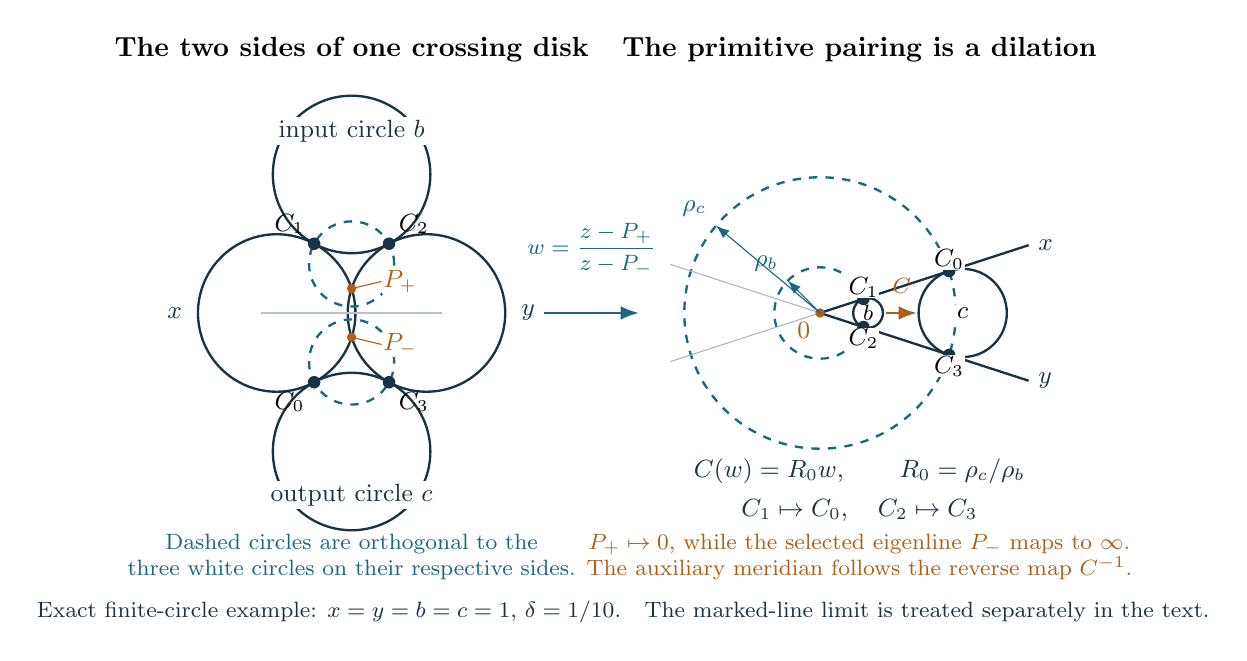
\begin{tikzpicture}[x=1cm,y=1cm,font=\small,>=Latex,
 whitecircle/.style={draw=ink,line width=.85pt},
 shadedcircle/.style={draw=blue,line width=.85pt,dashed},
 contact/.style={circle,fill=ink,inner sep=1.6pt}]
\pgfmathsetmacro{\ang}{18}
\pgfmathsetmacro{\s}{sin(\ang)}
\pgfmathsetmacro{\co}{cos(\ang)}
\pgfmathsetmacro{\len}{2*\co}
\pgfmathsetmacro{\u}{\co}
\pgfmathsetmacro{\qmid}{sqrt(4-\u*\u)}
\pgfmathsetmacro{\bb}{2+2*\s*\s}
\pgfmathsetmacro{\eb}{\bb+2*\s*\qmid}
\pgfmathsetmacro{\tb}{\bb/(2*\qmid)}
\pgfmathsetmacro{\rs}{sqrt(\tb*\tb-\s*\s)}
\pgfmathsetmacro{\rb}{\len/\eb}
\pgfmathsetmacro{\rc}{1/\rb}
\pgfmathsetmacro{\mb}{\rb/\co}
\pgfmathsetmacro{\mc}{\rc/\co}
\pgfmathsetmacro{\wb}{\rb*tan(\ang)}
\pgfmathsetmacro{\wc}{\rc*tan(\ang)}
\begin{scope}[shift={(1.1,3.25)}]
 \node[font=\bfseries] at (\u,3.35) {The two sides of one crossing disk};
 \draw[whitecircle] (0,0) circle (1);
 \draw[whitecircle] (\len,0) circle (1);
 \draw[whitecircle] (\u,\qmid) circle (1);
 \draw[whitecircle] (\u,-\qmid) circle (1);
 \draw[shadedcircle] (\u,\tb) circle (\rs);
 \draw[shadedcircle] (\u,-\tb) circle (\rs);
 \draw[ink!30] (-.2,0)--(\len+.2,0);
 \node[anchor=east,text=ink] at (-1.08,0) {$x$};
 \node[anchor=west,text=ink] at (\len+1.08,0) {$y$};
 \node[text=ink,fill=white,inner sep=1pt] at (\u,\qmid+.55) {input circle $b$};
 \node[text=ink,fill=white,inner sep=1pt] at (\u,-\qmid-.55) {output circle $c$};
 \coordinate (c1) at ({\u/2},{\qmid/2});
 \coordinate (c2) at ({(\len+\u)/2},{\qmid/2});
 \coordinate (c0) at ({\u/2},{-\qmid/2});
 \coordinate (c3) at ({(\len+\u)/2},{-\qmid/2});
 \foreach \p in {c0,c1,c2,c3} \node[contact] at (\p) {};
 \node[above left] at (c1) {$C_1$};\node[above right] at (c2) {$C_2$};
 \node[below left] at (c0) {$C_0$};\node[below right] at (c3) {$C_3$};
 \fill[amber] (\u,\s) circle (1.7pt);
 \fill[amber] (\u,-\s) circle (1.7pt);
 \draw[amber,thin] (\u,\s)--(\u+.38,.40);
 \draw[amber,thin] (\u,-\s)--(\u+.38,-.40);
 \node[anchor=west,text=amber,fill=white,inner sep=.5pt] at (\u+.38,.40) {$P_+$};
 \node[anchor=west,text=amber,fill=white,inner sep=.5pt] at (\u+.38,-.40) {$P_-$};
 \node[align=center,font=\footnotesize,text=blue] at (\u,-3.1)
 {Dashed circles are orthogonal to the\\three white circles on their respective sides.};
\end{scope}
\draw[->,thick,blue] (4.5,3.25)--(5.7,3.25);
\node[align=center,text=blue,font=\footnotesize] at (5.1,4.05)
 {$w=\dfrac{z-P_+}{z-P_-}$};
\begin{scope}[shift={(8.0,3.25)}]
 \node[font=\bfseries] at (.5,3.35) {The primitive pairing is a dilation};
 \draw[shadedcircle] (0,0) circle (\rb);
 \draw[shadedcircle] (0,0) circle (\rc);
 \draw[ink!35] (-1.9,{-1.9*tan(\ang)})--(0,0);
 \draw[ink!35] (-1.9,{1.9*tan(\ang)})--(0,0);
 \draw[whitecircle] (0,0)--(2.65,{2.65*tan(\ang)});
 \draw[whitecircle] (0,0)--(2.65,{-2.65*tan(\ang)});
 \node[right,text=ink] at (2.65,{2.65*tan(\ang)}) {$x$};
 \node[right,text=ink] at (2.65,{-2.65*tan(\ang)}) {$y$};
 \draw[whitecircle] (\mb,0) circle (\wb);
 \draw[whitecircle] (\mc,0) circle (\wc);
 \node[font=\footnotesize,fill=white,inner sep=1pt] at (\mb,0) {$b$};
 \node[font=\small,fill=white,inner sep=1pt] at (\mc,0) {$c$};
 \fill[amber] (0,0) circle (1.7pt);
 \node[below left,text=amber] at (0,0) {$0$};
 \foreach \sgn/\rad/\lab/\side in {1/\rb/C_1/above,-1/\rb/C_2/below,1/\rc/C_0/above,-1/\rc/C_3/below} {
  \coordinate (p) at ({\rad*\co},{\sgn*\rad*\s});
  \node[contact] at (p) {};
  \node[\side,fill=white,inner sep=.4pt] at (p) {$\lab$};
 }
 \draw[->,blue] (0,0)--({\rb*cos(135)},{\rb*sin(135)});
 \node[text=blue,above left] at ({\rb*cos(135)},{\rb*sin(135)}) {$\rho_b$};
 \draw[->,blue] (0,0)--({\rc*cos(140)},{\rc*sin(140)});
 \node[text=blue,above left] at ({\rc*cos(140)},{\rc*sin(140)}) {$\rho_c$};
 \draw[->,thick,amber] (.84,0)--(1.23,0);
 \node[text=amber,above,font=\footnotesize] at (1.04,.12) {$C$};
 \node[align=center,text=ink] at (.5,-2.25)
 {$C(w)=R_0w,\qquad R_0=\rho_c/\rho_b$\\[3pt]
  $C_1\mapsto C_0,\quad C_2\mapsto C_3$};
 \node[align=center,font=\footnotesize,text=amber] at (.5,-3.1)
 {$P_+\mapsto0$, while the selected eigenline $P_-$ maps to $\infty$.\\The auxiliary meridian follows the reverse map $C^{-1}$.};
\end{scope}
\node[font=\footnotesize,align=center,text=ink] at (5.5,-.55)
 {Exact finite-circle example: $x=y=b=c=1$, $\delta=1/10$.\quad
 The marked-line limit is treated separately in the text.};
\end{tikzpicture}
\end{document}
